\section{Introducción y Contexto Actual} \label{intro}

\noindent Hoy en día, prácticamente toda la información se almacena digitalmente y puede ser accedida en cualquier momento de manera sencilla. La mayoría de las personas están interconectados en todo momento con múltiples dispositivos mediante Internet, una plataforma cada vez más segura debido al trabajo de los especialistas, pero en la cual los delincuentes cibernéticos siguen encontrando vulnerabilidades y atacando todo tipo de entidades para conseguir beneficios \cite{STDWNCRY}. Hay muchos programas maliciosos como los virus, los gusanos informáticos y los troyanos que pueden dañar los sistemas digitales. Una de las principales amenazas cibernéticas en la actualidad, según un reporte de la agencia Europol \textit{(European Union Agency for Law Enforcement Cooperation)} \cite{3}, es el ransomware (rescate, en inglés ``ransom'', y ``ware'', acortamiento de software). Se trata de un tipo de malware que bloquea equipos o impide el acceso a los datos usando el cifrado de clave privada hasta que el usuario de dicho equipo paga un rescate, normalmente en \textit{bitcoin}. El robo de datos como extorsión lleva siendo utilizado desde alrededor de 2005, pero debido al auge del ransomware y el \textit{bitcoin}, se han incrementado enormemente el número de casos \cite{ZETTER}, con casi el 40\% de empresas habiendo sufrido al menos uno según un estudio realizado por Malwarebytes \cite{2}, lo que evidencia que estos programas maliciosos son una amenaza importante que hay que detectar y frenar cuanto antes.

Los delincuentes cibernéticos o ciberdelincuentes son cada vez más creativos e innovadores y, así mismo, el daño que causan va en aumento. En la Figura \ref{fig:im0-es} se muestra la predicción del coste de mitigación de daños frente a ataques ransomware para el año 2021, pudiendo apreciarse un gigantesco aumento respecto a la década pasada. Estos costes se deben tanto a la inversión para defender los sistemas, como a las pérdidas que se producen al no poder utilizar los equipos y al pago de los rescates.

\begin{figure}[h!]
\begin{center}
{\scalebox{.68}{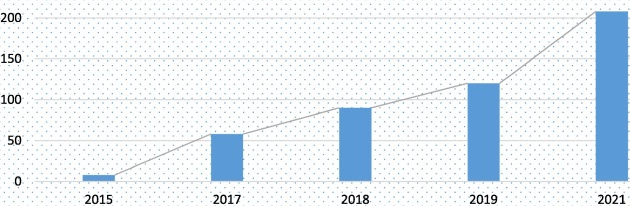
\includegraphics{images/grafica11.png}}}
\end{center}
\caption{Predicción del coste del ransomware en billones de dolares}
\label{fig:im0-es}
\end{figure}

%\change{verificar que los nombres de los labels es el mismo en la versi\'on en español e ingl\'es de la intro y conclusiones } HECHO

En la Figura \ref{fig:cove-es} se observa los resultados obtenidos de un estudio de Coveware \cite{4} sobre las industrias más afectadas por los ataques ransomware en el último trimestre del año 2020. Se puede apreciar que los servicios profesionales, el sector público y sanitario son los más afectados, ya que son los más rentables para los delincuentes. Esto se debe a su necesidad de estar en constante funcionamiento y por su posesión de datos delicados, por lo que suelen pagar los rescates para que se les devuelva sus datos y el acceso a sus sistemas lo más rápido posible.

\begin{figure}[h!]
\begin{center}
{\scalebox{.19}{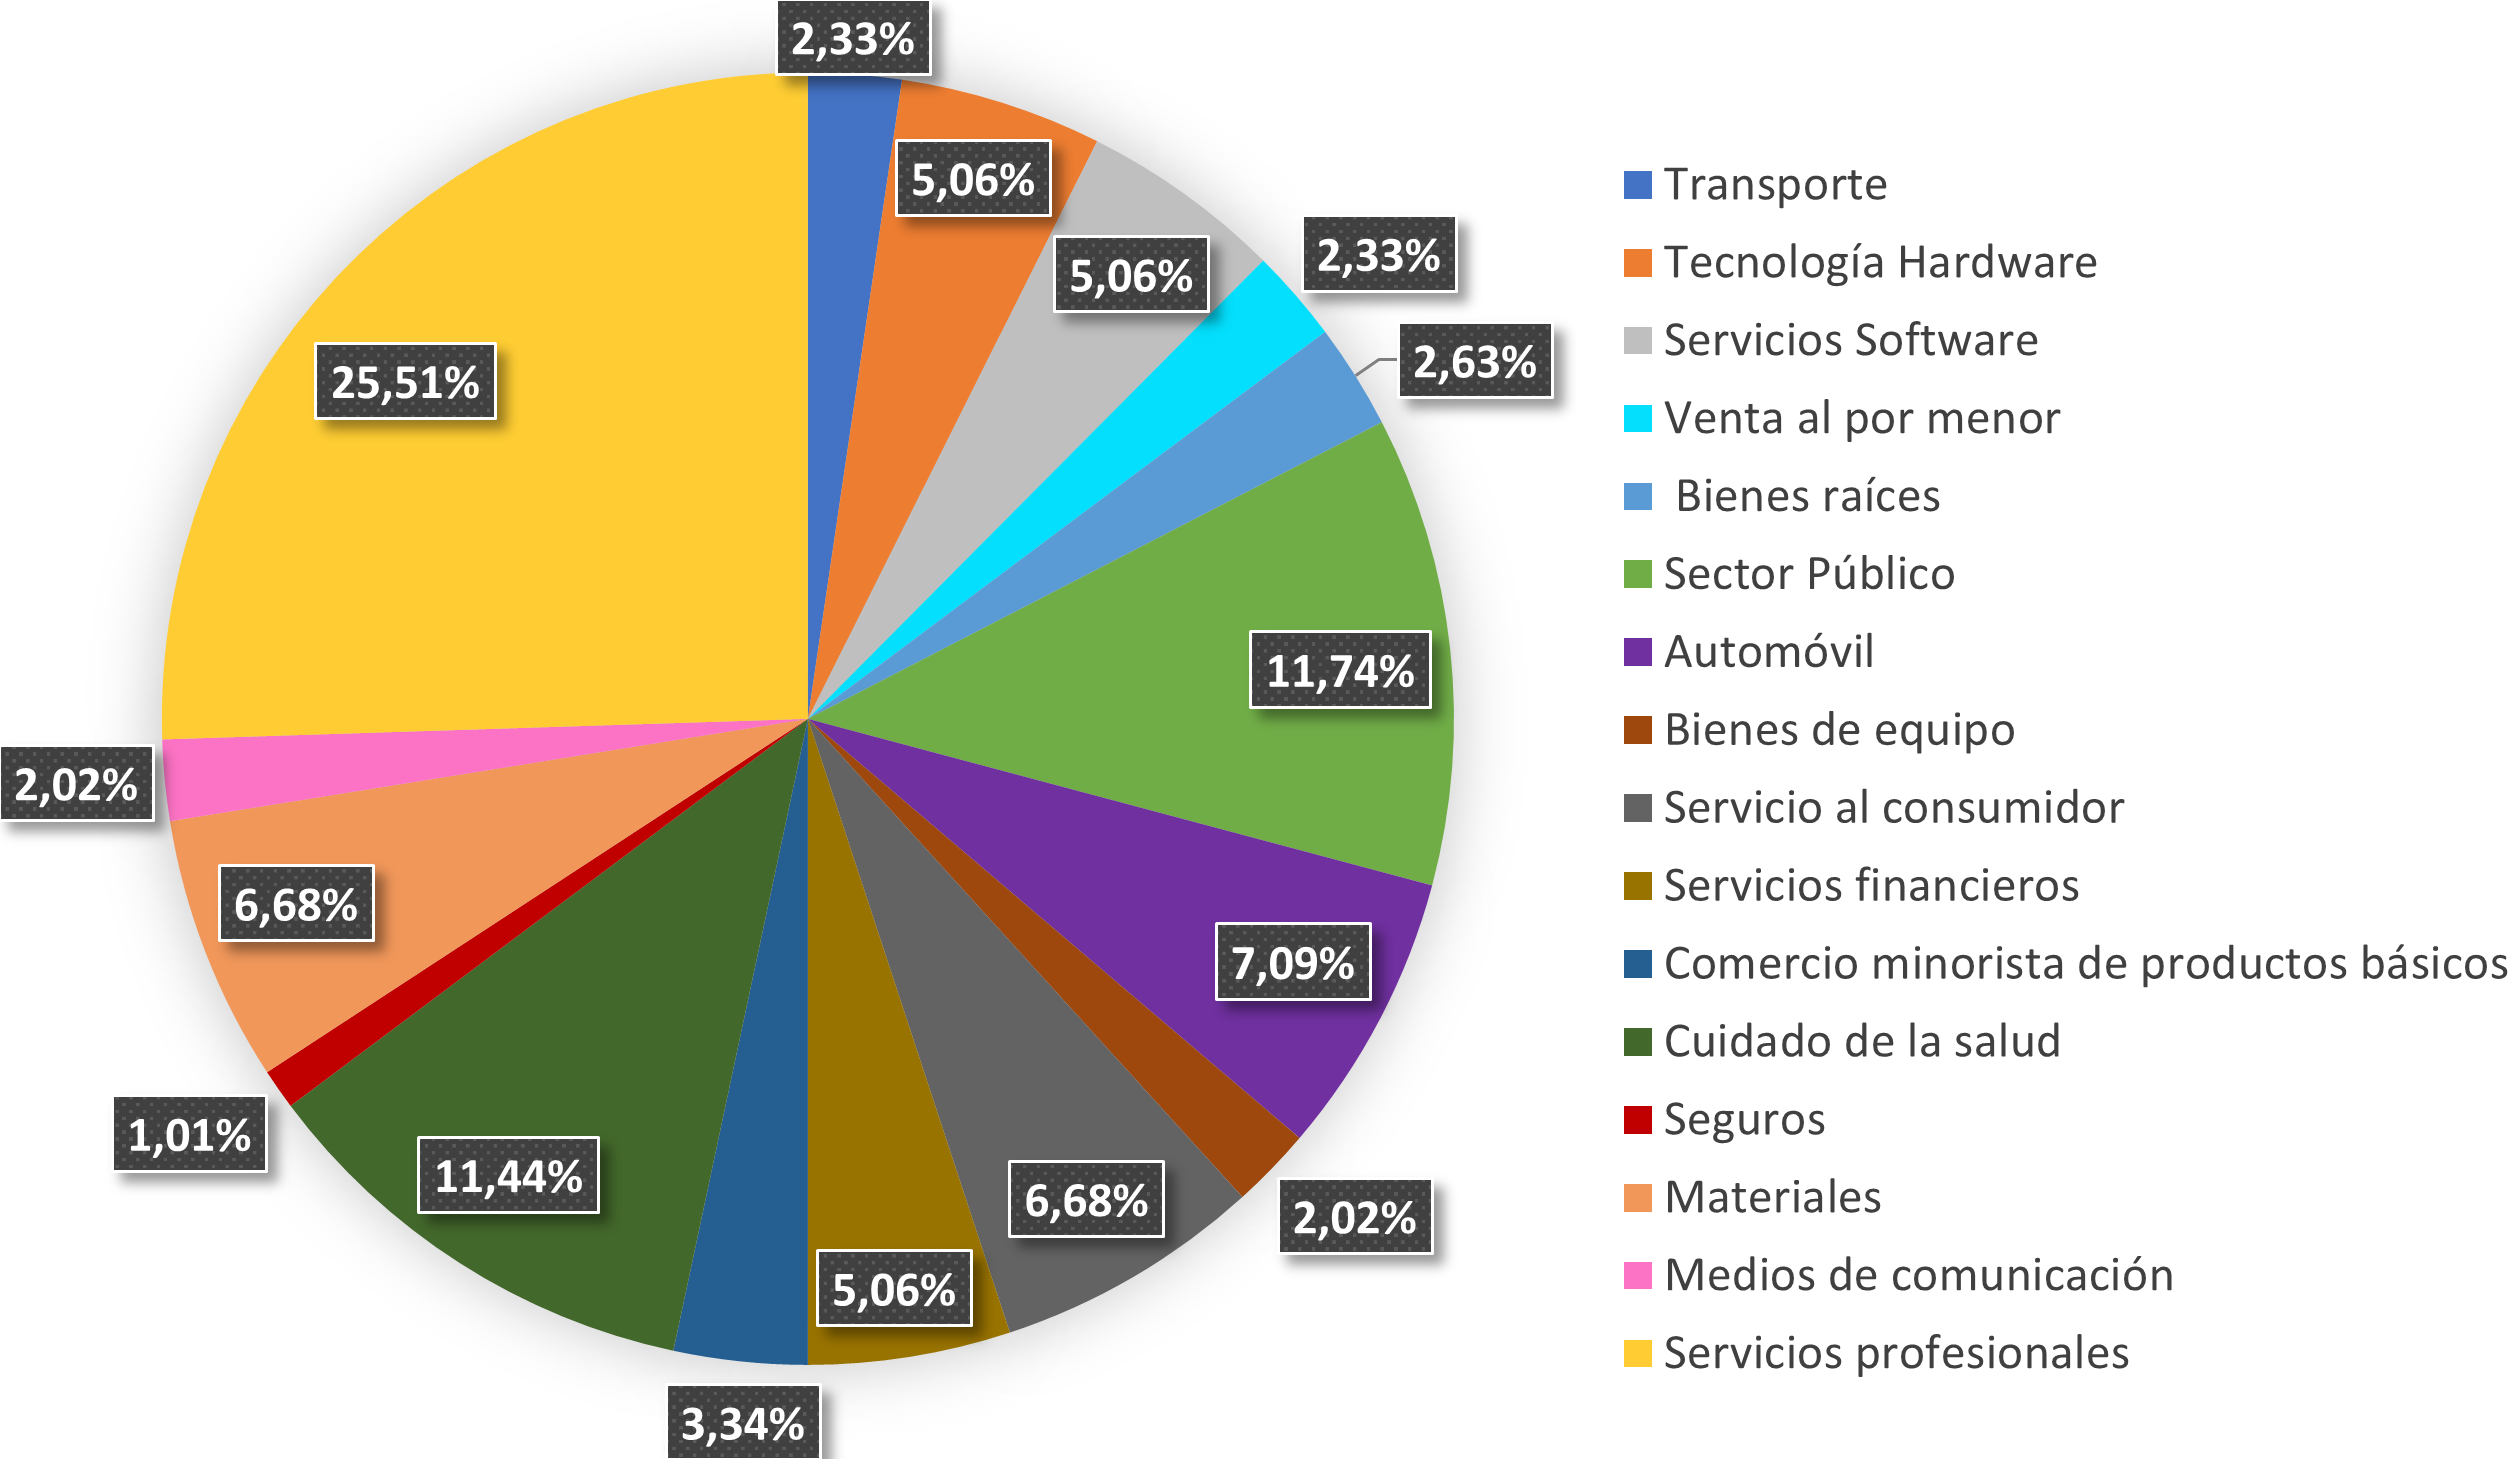
\includegraphics{images/industries2.png}}}
\end{center}
\caption{Sectores más atacados por ransomware en el tercer trimestre de 2020}
\label{fig:cove-es}
\end{figure}

El riesgo de un ciberataque es el mismo para una gran empresa que para una \gls{SME}. Estas compañías también utilizan, producen y almacenan grandes cantidades de datos. La diferencia es que las empresas más pequeñas han de lidiar con estos problemas con recursos mucho más limitados. Por lo tanto, deben hacer un mayor esfuerzo económico para trazar estrategias de seguridad ante estos ataques informáticos \cite{KURPJUHN20155}.

Al escenario planteado se le añade también la situación sanitaria actual, una la pandemia ocasionada por la enfermedad \gls{COVID-19}. Mientras esta se propagaba por el mundo, crecía una amenaza tecnológica secundaria basada en ciberataques indiscriminados y cibercampañas centradas en autoridades públicas y organizaciones \cite{LALLIE2021102248}, así como en los individuos basándose en su desinformación y temor, como la falsa distribución de libros con información sobre el \gls{COVID-19} \cite{MALWLABS}, la oferta fraudulenta de medicamentos vía correo electrónico \cite{NORTON}, etc.
Otro factor que ha favorecido el aumento de ciberataques, y en concreto, de ataques ransomware, es el establecimiento del teletrabajo. En España, estos tipos de ataques aumentaron un 160\% en el segundo semestre del año 2020, encabezando el \textit{ranking} europeo, debido a que las empresas que centraron sus esfuerzos en establecer entornos de trabajo a distancia, no aplicaron la seguridad necesaria para ello \cite{ELPAIS}. En España, las únicas empresas afectadas no han sido solo las privadas, ya que, por ejemplo, instituciones públicas recibieron ataques ransomware. El \gls{SEPE} tuvo que paralizar la totalidad de sus servicios durante 5 días, añadiendo otras 20 jornadas sin permitir el teletrabajo por un ataque en marzo de 2021 por el ransomware Ryuk, provocando una grave situación, pues la actividad del \gls{SEPE} se había disparado por el impacto de la pandemia en el desempleo \cite{RYUKSEPE}.


El desarrollo de la tecnología proporciona beneficios y facilidades en todos los ámbitos y tareas, hasta en los más cotidianos. Ejemplo de ello es el Internet de las Cosas, o \gls{IoT}, que se define como la integración de lugares y objetos de la vida real con Internet, mediante la interconexión de dispositivos, sensores, actuadores, software, etc. mediante una red, que almacena e intercambia información \cite{IoTDEF}. Sin embargo, la existencia de esta tecnología ha permitido que la cantidad de ataques ransomware crezcan con el tiempo, especialmente tras el incremento del uso de dispositivos \gls{IoT} inteligentes, particularmente los móviles. En la Figura \ref{fig:im1-es} se puede observar la cantidad de ataques ransomware a dispositivos móviles por trimestre en 2018. La Figura \ref{fig:im2-es} muestra una predicción del incremento del uso de este tipo de dispositivos debido al auge del \gls{IoT}. Con estos datos se puede predecir que la cantidad de ataques continuará en alza y se demuestra que existe una necesidad tanto de proteger a los individuos y las organizaciones de esta clase de ataques como de ofrecer la información existente a los usuarios y trabajadores  para actuar de una forma responsable y segura para prevenirlos \cite{HUMAYUN2021105}.

% IMAGEN 1
\begin{figure}[htb]
\begin{center}
{\scalebox{.4}{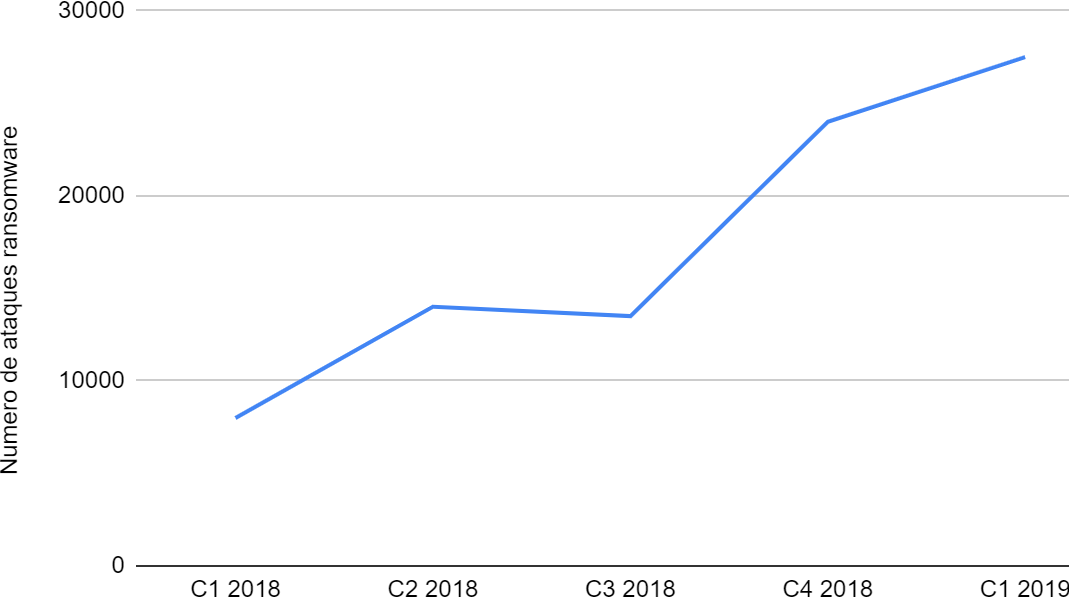
\includegraphics{images/grafica4.png}}}
\end{center}
\caption{Ataques ransomware a dispositivos móviles}
\label{fig:im1-es}
\end{figure}


% IMAGEN 2
\begin{figure}[htb]
\begin{center}
{\scalebox{.6}{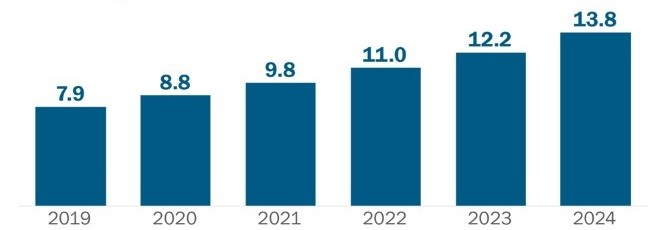
\includegraphics{images/grafica31.jpg}}}
\end{center}
\caption{Predicción de la cantidad de dispositivos IoT móviles en miles de millones}
\label{fig:im2-es}
\end{figure}


\section{Motivación}
\noindent Como se ha visto en la Sección \ref{intro}, es evidente el impacto de los ataques ransomware en las empresas en los últimos años, provocando grandes inversiones económicas para mejorar la seguridad.
Las \gls{SME} tienen mayor dificultad para afrontar dichos gastos y por lo tanto están más expuestas, debido a que no tienen sistemas de prevención, especialistas enfocados en la ciberseguridad e incluso información relativa a este sector.

En la Unión Europea, las \gls{SME} constituyen un pilar fundamental de la economía, representando en septiembre de 2020 un sorprendente 99,8\% de todas las empresas empleadoras, el 65\% del empleo del sector privado y el 54\% del sector privado de producción bruta. 
Éstas han sido además muy vulnerables a la pandemia ocasionada por el \gls{COVID-19}, provocando grandes pérdidas e incluso gran cantidad de cierres \cite{NBER}. 
Debido a todos estos factores, la motivación principal de este estudio es el desarrollo de un modelo de detección de ransomware que cumpla con los siguientes requisitos: Precisión, fiabilidad, escalabilidad, facilidad de uso, rapidez y software libre.

De esta manera se puede llevar a cabo una estrategia de prevención contra ataques ransomware y reducir el impacto de los daños ocasionados por ellos a través de una herramienta accesible a las \gls{SME}, reduciendo de manera drástica los costes de inversión.


%\section{Contexto}
%\noindent Este Trabajo Fin de Grado ha sido realizado dentro del Grupo de Análisis, Seguridad y Sistemas (Grupo GASS \cite{GASS01}, \url{https://gass.ucm.es/}, Grupo 910623 del catálogo de grupos reconocidos por la \gls{UCM}) como parte de un proyecto de investigación aprobado por la Comisión Europea. %decir que nos digan detalles de esto


\section{Objetivos}
\noindent Al inicio del trabajo, se establecen una serie de objetivos para asegurar su calidad y fijar unas pautas para el correcto desarrollo:
\begin{itemize}
    \item Utilizar las competencias adquiridas durante el grado.
    \item Desarrollar un modelo de \gls{ML} capaz de identificar muestras de ransomware con gran precisión.
    \item Construir un extenso \textit{dataset} para garantizar la fiabilidad en los resultados obtenidos. 
    \item Desarrollar y desplegar un laboratorio para el análisis de muestras de malware.
    \item Demostrar la efectividad de las llamadas a las \gls{API} de Windows de un ejecutable como mecanismo de detección de ransomware. %Comprobar, a su vez, la mejora del comportamiento al utilizar la cantidad de llamadas en lugar de su aparición única. %yo esto lo quitaria
\end{itemize}


\section{Plan de Trabajo}
\noindent El desarrollo de este trabajo se ha realizado en las siguientes fases:
\begin{enumerate}
    \item \textbf{Investigación}: Esta fase se llevó a cabo durante los primeros cuatro meses, donde se adquirió la información necesaria para el desarrollo del trabajo. Al comienzo de la fase, se realizaron varias reuniones donde se explicaron los objetivos del proyecto y los conocimientos necesarios, siendo estos los conceptos fundamentales del aprendizaje automático. Una herramienta primordial para la investigación fue \textit{Google Scholar}, ya que permite buscar artículos científicos y citarlos con facilidad. Se buscaron artículos y publicaciones sobre detección tanto de ransomware como de malware, además de libros sobre análisis malware para adquirir conocimientos más profundos del tema y entender el contexto del trabajo.
    \item \textbf{Desarrollo}: Una vez obtenidos los conocimientos necesarios, se comenzó el desarrollo del modelo. No se abandonó por completo la investigación, pero pasó a un segundo plano. Durante esta fase se obtuvieron los datos necesarios y se construyeron los dos \textit{datasets} para entrenar y evaluar el modelo propuesto. Posteriormente se pasó a la familiarización con el lenguaje de programación Python y con la librería \textit{scikit-learn}, usada para la codificación del modelo y la implementación de los algoritmos de \gls{ML}.
    \item \textbf{Experimentación y resultados}: En esta fase experimentó con el modelo desarrollado y los datos extraídos. Al obtener los resultados era necesario evaluarlos y demostrar la validez del modelo, por lo que se usó la validación cruzada K-Fold. La experimentación fue vital para la fase de desarrollo, ya que se tuvo que modificar el modelo para mejorar los resultados, ajustando los parámetros, obteniendo más datos...
    \item \textbf{Documentación}: La fase de documentación se llevó a cabo de manera paralela al resto de fases. Empezó en los últimos meses de la fase de investigación con los conocimientos asentados, y continuó durante el desarrollo y la experimentación. Todos los miembros del equipo participaron en la escritura de la memoria, trabajando en conjunto en todas las secciones. Cualquier actualización debía de ser aceptada y revisada por los otros miembros del equipo.
\end{enumerate}

El modelo desarrollado en este trabajo está subido en el repositorio de Gitlab \href{https://gitlab.fdi.ucm.es/marina.lopez/tfg-ransomware-20-21}{TFG Ransomware 20-21}.


%\change{Agregar las actividades realizadas en y el diagrama de Gannt}
La Figura \ref{fig:gantt} es un diagrama de Gantt donde se pueden apreciar las actividades desempeñadas por el equipo a lo largo de los meses y su duración.

\begin{figure}[htb]
\begin{center}
{\scalebox{.9}{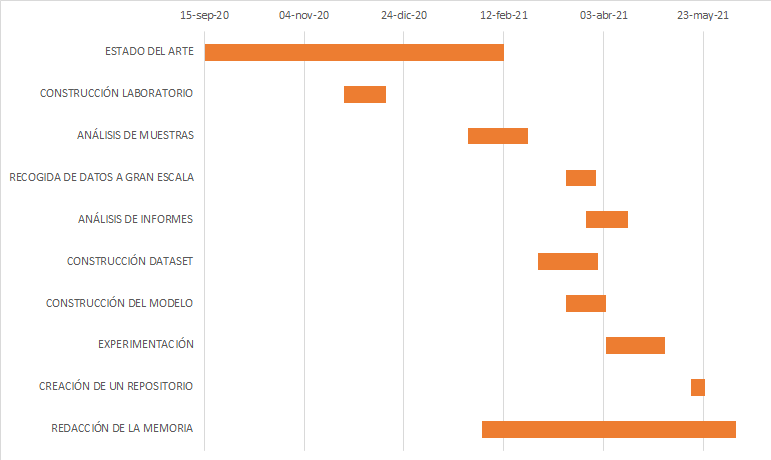
\includegraphics{images/gant.png}}}
\end{center}
\caption{Diagrama de Gantt de las tareas desempeñadas.}
\label{fig:gantt}
\end{figure}

\section{Estructura del Trabajo}
\noindent El resto del trabajo está organizado en 10 capítulos, siguiendo esta estructura:

%\Ransomware
El Capítulo \ref{Capitulo2} introduce el ransomware, explicando los conceptos fundamentales sobre el malware y los diferentes tipos, el modelo de negocio que siguen los ciberdelincuentes para sacar beneficio de los ataques y la evolución histórica del ransomware, detallando cada año los diferentes ataques que han habido en el mundo. También se exponen los diferentes tipos de ransomware, las familias, los métodos de propagación más comunes y posteriormente el modo de operación para infectar el sistema de la víctima. El capítulo termina explicando algunas técnicas usadas por programas antivirus para reconocer la presencia del ransomware y unas estrategias y acciones de prevención que toda empresa debería seguir para proteger sus sistemas de estos ataques, y en caso de sufrirlos, que pasos deberían seguir para recuperas sus datos.

%Análisis e identificación de malware
El Capítulo \ref{Capitulo3} aborda los tipos de análisis de malware que existen, las herramientas que se usan, las limitaciones de cada uno y las diferentes técnicas de identificación. Posteriormente se habla del aprendizaje automático aplicado al análisis malware, exponiendo cómo se construye un modelo de \gls{ML} usando Python como lenguaje de programación y los diferentes algoritmos que existen, indagando en los denominados algoritmos de aprendizaje supervisado, ya que son los que más se utilizan en análisis y detección de malware y ransomware.

%Estado del arte
El Capítulo \ref{Capitulo4} se muestran trabajos relacionados con el tema de análisis y detección de malware y ransomware usando modelos de \gls{ML} y algoritmos de aprendizaje automático. Se distinguen entre trabajos que solo analizan malware de los que analizan ransomware, y dentro de los trabajos de ransomware se diferencian los que usan las llamadas a la \gls{API} de Windows para construir sus modelos de los que no.

%Arquitectura y tecnologías utilizadas (Sistema Propuesto)
El Capítulo \ref{Capitulo5} expone las tecnologías usadas para desarrollar el modelo de \gls{ML}, el entorno de trabajo y la obtención de los datos. Se muestra el diagrama de flujo del sistema propuesto y se habla sobre el desarrollo del laboratorio de análisis para el estudio de las muestras de ransomware y goodware, de las cuales se extraen las llamadas a la \gls{API} de Windows para la construcción de los \textit{datasets}. Posteriormente se hace una limpieza de los datos en los \textit{datasets} para descartar aquellos que no son relevantes para el estudio y se explica cómo se creará el modelo.

%Experimentos y resultados
El Capítulo \ref{Capitulo6} aborda los experimentos realizados y las métricas utilizadas para demostrar la efectividad del modelo para detectar ransomware. Después de mostrar los experimentos sobre los dos \textit{datasets} y los parámetros utilizados para su desarrollo, se obtienen los resultados finales y se validan con la validación cruzada K-fold. Posteriormente se elige el algoritmo que mejores resultados ha obtenido y se comparan con los resultados de los trabajos relacionados expuestos en el Capítulo \ref{Capitulo4}.

%Conclusiones y trabajo futuro
El Capítulo \ref{Capitulo7} muestra las conclusiones del trabajo tras el análisis de los resultados y expone las líneas de investigación futuras.

%Contribucion de cada uno
El Capítulo \ref{Capitulo8} relata las aportaciones individuales de cada miembro del equipo al desarrollo del trabajo.

%Ingles
Los Capítulos \ref{Capitulo9} y \ref{Capitulo10} son las traducciones al inglés de los Capítulos \ref{Capitulo1} y \ref{Capitulo7}.